\documentclass[a4paper, 11pt, oneside, openright, english]{book}
\usepackage[utf8]{inputenc}
\usepackage{graphicx}
\usepackage{hyperref}
\usepackage{booktabs}
\usepackage{blindtext}
\usepackage{amsmath}
\usepackage{amssymb}
\usepackage{listings}
\usepackage{titlesec}
\usepackage{xcolor}
\usepackage{longtable}
\usepackage{seqsplit}
\usepackage{geometry}
\usepackage{fancyhdr}
\usepackage{float}
\usepackage{longtable}
\usepackage{enumitem}

\pagestyle{fancy}
\fancyhf{}

\fancyhead[LE,RO]{\slshape \rightmark}
\fancyhead[LO,RE]{\slshape \leftmark}
\fancyfoot[C]{\thepage}
\renewcommand{\chaptermark}[1]{\markboth{#1}{}}
\renewcommand{\sectionmark}[1]{\markright{\thesection.\ #1}}

\setlength{\headheight}{13.59999pt}
\addtolength{\topmargin}{-1.59999pt}

\titleformat{\chapter}[block]{\normalfont\huge\bfseries}{\thechapter.}{1em}{\Huge}

\begin{document}
\input title 
\input revision_history
\tableofcontents

\chapter{Introduction}

\section{Purpose}
The purpose of this document is to present a detailed description of CodeKataBattle (CKB).
It provides functional and non-functional requirements for the development of the system, including use cases, features, user interaction and system constraints. This document is addressed to the developers who have to implement the requirements and
could be used as an agreement between the customer and the contractors.

CodeKataBattle (CKB) is a new platform that helps students improve their software development skills by training with peers on code kata. Educators use the platform to challenge students by creating code
kata battles in which teams of students can compete against each other, thus proving (and improving) their skills and soft-skills : in fact working in a team is useful to learn soft-skills such as
communication and coordination.

A code kata battle is essentially a programming exercise in a programming language of choice (e.g.,
Java, Python). The exercise includes a brief textual description and a software project with build
automation scripts (e.g., a Gradle project in case of Java sources) that contains a set of test cases that
the program must pass, but without the program implementation. Students are asked to complete the
project with their code. In particular, groups of students participating in a battle are expected to follow
a test-first approach and develop a solution that passes the required tests. Groups deliver their
solution to the platform (by the end of the battle). At the end of the battle, the platform assigns scores
to groups to create a competition rank.

\subsection{Goals}
% \par\noindent\rule{
% \begin{table}[h]
%     \begin{tabular}{ c p{2cm} }
%         \hline
%         \textbf{G1} & Allows Students to improve their software development skills by partecipating in coding tournaments where they write programs \\
%         \textbf{G2} & Allows Educators to challenge Students by create coding tournaments and battles.                                              \\
%         \hline
%     \end{tabular}
%     \label{tab:Goals}
% \end{table}
% }

\begin{description}
    \item \textbf{G1} \quad Allows Students to improve their software development skills by partecipating in coding tournaments where they write programs
    \item \textbf{G2} \quad Allows Educators to challenge Students by create coding tournaments and battles.
    \item \textbf{Gi} \quad Allows Educators to track Students' knowledge about software development, evaluating the code written during battles and the overall score obtained in tournaments
    \item \textbf{Gi} \quad Allows Educators to customize battles defining specific rules, achivements that Students can obtain and evaluation modality.
    \item \textbf{Gi} \quad Allows Students to improve their soft skills, as communication, collaboration and time management, by creating teams for coding battles
    \item {\textcolor{red}{Non son sicuro siano goal che Code kata vuole risolvere}}
    \item \(G_i\) Allows S to learn sw develoment divertendosi e confrontandosi con i compagni in sane competizioni con ranking
\end{description}
\par\noindent\rule{\textwidth}{0.5pt}

\blindtext
\section{Scope}

{\color{red} In another RASD here there are a few words}

\subsection{World Phenomena}
\par\noindent\rule{\textwidth}{0.5pt}
\begin{description}
    \item \textbf{WP1} \quad The students fork the GitHub repository of the code kata
    \item \textbf{WP1} \quad Students set up an automatic workflow in the GitHub repository
    \item \textbf{WP1} \quad The students work on the code kata battle
    \item \textbf{WP1} \quad The students push their work to the GitHub repository
    \item \textbf{WP1} \quad An educator upload correct test cases and automation scripts
    \item \textbf{WP1} \quad An educator evaluates the work done by the team at the end of the code kata battle
\end{description}
\par\noindent\rule{\textwidth}{0.5pt}


\subsection{Shared Phenomena}
\begin{description}
    \item \(SP_i\) An educator creates a tournament
    \item \(SP_i\) An educator grants other colleagues permission to create battles
    \item \(SP_i\) An educator creates a battle within a tournament
    \item \(SP_i\) The students are notified of a new tournament
    \item \(SP_i\) The students are notified of a new upcoming battle within a tournament they are subscribed to
    \item \(SP_i\) Students use the platform to form teams
    \item \(SP_i\) Student invite other students to join its team respecting the boundaries imposed
    \item \(SP_i\) Student join a battle on his own
    \item \(SP_i\) Student join a battle towards an invite -> Possono scegliere di essere soli oppure devono per forza
    \item \(SP_i\) The platform sends the link of the GitHub repository to all students who are members of subscribed teams
    \item \(SP_i\) Students are asked to fork the GitHub repository and set up an automated workflow
    \item \(SP_i\) The forked repository's workflow notifies the platform of a new push
    \item \(SP_i\) The platform updates the battle score of a team
    \item \(SP_i\) The educator uses the platform to go through the sources produced by each team
    \item \(SP_i\) The educator assigns additional score to the teams after the evaluation
    \item \(SP_i\) The platform notifies the teams when the final battle rank becomes available
    \item \(SP_i\) The platform updates the personal tournament score of each student
    \item \(SP_i\) An educator closes a tournament
    \item \(SP_i\) The platform notifies all students involved in the tournament about its end
    \item \(SP_i\) All users see the list of  ongoing tournaments as well as the corresponding tournament rank
    \item \(SP_i\) An educator defines the gamification badges
    \item \(SP_i\) Student visualize gained badges on its profile
\end{description}

\section{Definitions, Acronyms, Abbreviations}
\subsection{Abbreviations}
\(G_i\) = i-th goal \\
\(WP_i\) = i-th World Phenomena\\
\(SP_i\) = i-th Shared Phenomena\\

\subsection{Acronyms}
E = educator \\
S = students
\section{Revision history}
\section{Reference Documents}
Assign document for A.Y. 2023-2024 "Requirement Engineering and Design Project: goal, schedule, and rules"

\section{Document Structure}
The structure of this RASD document follows six main sections:
\begin{enumerate}
    \item \textbf{Introduction:}
          provides an overview of the problem at hand, the purpose of the document and
          the project, the scope of the domain, and introduces the main goals of the system as a solution.

    \item \textbf{Overall Description:}
          gives a general description of the system, going into more details about its main functions.
          The description is assisted with the help of UML diagrams, such as class, activity and state diagram.
          The domain assumptions of the examined world are then explained along with any dependencies and constraints.

    \item \textbf{Specific Requirements:}
          

    \item \textbf{Formal Analysis Using Alloy:}

    \item \textbf{Effort Spent:}
          keeps track of the time spent to complete this document.
          The first table defines the amount of hours used by the whole team to get important decisions and to make reviews,
          the other tables contains the individual effort spent by each team member.

    \item \textbf{References:}
          lists all the documents used and that were helpfull in drafting the RASD.
\end{enumerate}
\chapter{Overall Description}
\section{Product Perspective}
\subsection{Scenarios}

\subsubsection{Creating a tournament}
Chip, a professor of Algorithm and Data Structures at Mouseton Institute of Technology, prepared to teach the chapter on strings, launching the "Strings Operations" coding tournament on CKB.
To expand participation, he allowed his colleague Dale to create challenges for his software engineering class.
Students across classes would compete in string manipulation tasks, ranging from basic concatenation to advanced text analysis, fostering collaboration and learning.
To make the tournament more interesting, Chip decided to award badges to the best performing students, so he created a badge for the student who participated in the most tournaments, one for the student who won the most battles and one for the student that wrote the most lines of code.
All students already subscribed to CKB were notified of the new tournament, and they could join it from the tournament page.

\subsubsection{Creating a battle}
In order to get the students familiar with the CKB platform and its features, Chip created an easy battle for his students to practice on, called "wordcheck", that basically requires the student to implement the game wordle.
He decides that the battle will last 2 weeks and that the students will be able to work in teams of 2 or 3 people; they will be able to join the battle until the last day of the battle.
In addiction, he wants to give extra points to the code cleanup, so he will have to revise the code of each team at the end of the battle and assign extra points to the teams that wrote clean code.
He sets all this information in the battle creation form and then he creates the battle.

\subsubsection{Joining a battle}
Huey and Dewey, two students of Chip's class, are notified of a new battle and decide to join it.
Since the the more the merrier, they decide to invite their friend Louie to join them in the battle.
After the registration deadline, they are notified that the battle is about to start and they are given the link to the GitHub repository of the battle to fork and set up the automated workflow in order to be able to link their GitHub account to the CKB platform.
After the automated workflow is set up, they are ready to start working on the battle.

\subsubsection{Improving the score and obtaining a badge}
Donald is a warrior of the "wordcheck" battle and he is working on the battle alone.
After a fitst commit, he logs in to the CKB to check his score.
He sees that he is in the 3rd position and that he is 10 points behind the leader group, that is composed by Huey, Dewey and Louie.
Fortunately, the battle is still open and the CKB platform allows him to improve his score by pushing new commits to the GitHub repository, so he decides to work on the battle for a couple of days and then push his work to the GitHub repository.
After checking his score again, he sees that he is now in the 1st position and moreover he obtained a badge for being the first to reach 100 points in the battle and now both students and professors can see this badge when they visit Donald's profile.

\subsubsection{Closing a battle}
When the deadline for the battle created by Scrooge is reached, all participants are notified that the battle is closed and that they can't push new commits to the GitHub repository.
Scrooge is notified that the battle is closed and he can now evaluate the code of each team and assign extra points for the clarity of the comments and the code, as he decided when he created the battle.
After the evaluation, the final rank of the battle is available to all participants and the students are notified that they can now see the final rank of the battle.

\subsubsection{Closing a tournament}
Chip decides to close the "Strings Operations" tournament, even if the deadline is not reached yet.
In order to do so, he logs in to the CKB platform and he closes the tournament.
All participants are notified that the tournament is closed and that they can't join it anymore, in the end, the CKB platform makes the final rank of the tournament available to all participants.

\subsubsection{Accessing the scores of the players}
Huey wishes to enroll to the class of Advanced Algorithms and Data Structures held by professor Pippo, so he applies for the class.
Pippo, who wants to make sure that Huey is a good student, comes to know that Huey is a very active user of the CKB platform and he decides to check his profile.
He sees that Huey has a very high score in the "Strings Operations" tournament and that he has a badge for being the most active user of the platform and he also notes that Huey is involved in more than one tournament simultaneously.
Thanks to the CKB platform, Pippo has now a complete overview of Huey's skills and he can decide whether to accept his application or not.

\subsection{\textcolor{red}{Class Diagram}}

\subsection{State Diagrams}
The following state diagrams describe the life cycle of the main entities of the system.
Moreover, they also specify the sequence of states that an object goes through during its lifetime in response to stimuli from the environment.
We want to focus on the events that cause a transition from one state to another and the actions that result from a state change.

\subsubsection*{Tournament}
After an educator creates a tournament, it is both in the \textit{registration open} and \textit{tournament open} states.\\
In the \textit{registration open} state, students can join the tournament, while in the \textit{tournament open} state, educators with the right permissions can create battles within the tournament, and that leads the tournament to the \textit{battling} state.\\
When the deadline for the registration is reached, the tournament moves to the \textit{registration closed} state and no more students can join it.\\
When the deadline for the registrations is reached, no more students can join the tournament and it moves permanently to the \textit{registration clcsed} state.\\
During the \textit{battling} state educatos can start multiple parallel battles and, if and only if all battles are ended, the educator can finally close the tournament.\\
The diagram is shown in figure \ref{fig:tournament-state-diagram}.\\

\subsubsection*{Battle}
The battle evolves in a linear way, starting from the \textit{registration opem} immediately followed by the \textit{registration closed} state.\\
After the registration deadline is reached, the github repository of the battle is created and thus the battle moves to the \textit{coding} state, allowing the students to fork the repository and start working on the battle.\\
When the deadline for the battle is reached, the educators can start evaluating the code of the students, if previously enabled (\textit{consolidation} state). \\
After the evaluation is completed, the battle can be closed and the final rank is available to all participants.\\
The diagram is shown in figure \ref{fig:battle-state-diagram}.\\

\subsubsection*{Score evaluation}
The score evaluation is a process that is triggered by the end of a battle and it is composed by multiple steps.\\
First, three aspects can be automatically evaluated: functional aspects (the higher the better, +), timeliness (the lower the better, -) and quality level of the sources, extracted through static analysis tools (+). \\
Finally, if the educator enabled the manual evaluation, he can assign extra points. \\
The diagram is shown in figure \ref{fig:score-evaluation-state-diagram}.\\

\begin{figure}[H]
    \centering
    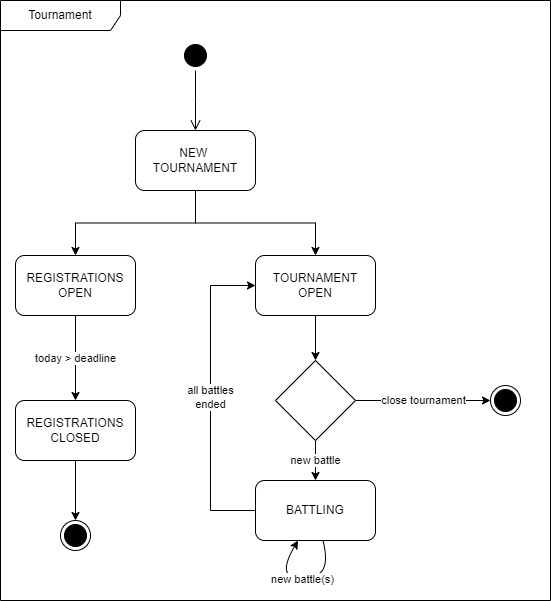
\includegraphics[width=0.8\textwidth]{state_diagrams/tournament.jpg}
    \caption{Tournament state diagram}
    \label{fig:tournament-state-diagram}
\end{figure}
\begin{figure}[H]
    \centering
    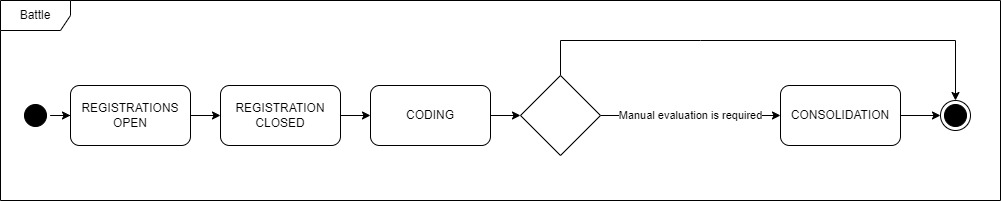
\includegraphics[width=0.8\textwidth]{state_diagrams/battle.jpg}
    \caption{Battle state diagram}
    \label{fig:battle-state-diagram}
\end{figure}
\begin{figure}[H]
    \centering
    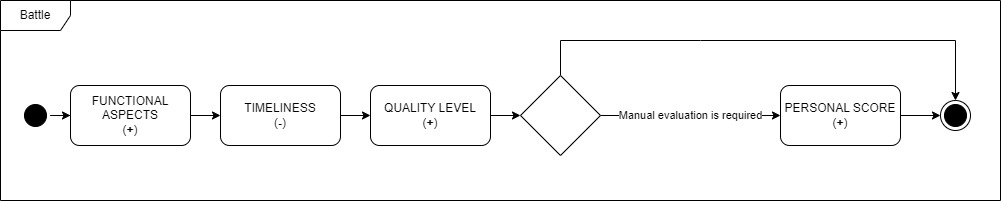
\includegraphics[width=0.8\textwidth]{state_diagrams/score_evaluation.jpg}
    \caption{Score evaluation state diagram}
    \label{fig:score-evaluation-state-diagram}
\end{figure}

{\color{red}
\section{Product Functions}
\section{User characteristics}
\section{Assumptions, Dependencies and Constraints}
\subsection{Domain Assumptions}
\newlist{assumptionsenumerate}{enumerate}{1}
\setlist[assumptionsenumerate,1]{label=\textbf{D}\arabic*., ref=D\arabic*}
    \begin{assumptionsenumerate}
        \item STDs code with the programming language setted for the kata battle to which they are partecipating
        \item EDUs upload the code kata with the description and software project, including test cases and build automation scripts
        \item STDs fork the GitHub repository of the code kata and set up an automated workflow through GitHub Actions that informs the CKB platform (through proper API calls) as soon as STDs push a new commit into the main branch of their repository
        \item EDUs manual evaluation range from 0 to 100
        \item The information inserted at registration moment of all users are truthful
        \item GitHub and Gradle works properly
    \end{assumptionsenumerate}
\subsection{Dependencies}
}
\subsection{Constraints}

\begin{itemize}
    \item The software must follow local laws and rules, especially when it comes to handling user data, like letting users access their data when they want.
    \item The software should only collect the data it really needs, like just the user's email address.
    \item To keep users' important info safe, like passwords, it must be stored in SHA256 encoding in the database.
    \item When choosing external APIs, especially those that are crucial for it to work properly, we should pick the ones that are the most dependable and always available.
\end{itemize}
\chapter{Specific Requirements}

\section{External Interface Requirements}
In the following, the interfaces, both hardware and software, of the system are described.

    {\color{red}\subsection{User Interfaces}}

\subsection{Hardware Interfaces}
To use the CKB platform, both the Educators and the Students need an electronic device connected to the Internet, like a computer, a tablet or a smartphone.\\
As the platform's primary functionality is closely tied to coding activities, it is expected that users will predominantly employ personal computers to access an Integrated Development Environment (IDE). Consequently, the platform's interfaces have been optimized for use on computer screens.\\

\subsection{Software Interfaces}
Since the platform is web-based, it is compatible with all the major operating systems, as long as they have a modern browser installed.

\subsection{Communication Interfaces}
The system requires a stable internet connection to work properly. The backend of the system will expose a unified RESTful API to communicate with all clients.\\
Furthermore, he system relies on various external interfaces accessible via uniform web API. These services are:
\begin{itemize}
    \item \textbf{GitHub API:} to create and manage repositories and to retrieve the code of the students and to authenticate users.
    \item \textbf{Mail API:} to send emails to the users to notify them about events.
\end{itemize}

{\color{red} \section{Functional Requirements}}
In order to work properly, the software must fulfill the following functional requirements:
    \begin{requirements}
        \item \textbf{Ri} \quad The software shall allow the students to create an account
        \item \textbf{Ri} \quad The software shall allow the educators to create an account 
        \item \textbf{Ri} \quad The software shall allow the students to login
        \item \textbf{Ri} \quad The software shall allow the educators to login
        \item \textbf{Ri} \quad The software shall allow the educators to create new tournaments
        \item \textbf{Ri} \quad The software shall allow an educator to grant to other colleagues the permission to create battles
        \item \textbf{Ri} \quad The software shall allow the educators allowed for a specific tournament to create coding kata battles in a that specific tournament by letting them uploading the code kata, setting minimum and maximum number of students per group, setting a registration and a final submission deadlines, setting score configurations
        \item \textbf{Ri} \quad The software shall allow the students to form teams {\color{red} Penso che dovrei essere più specifico e dire come creare i team ma d'altro canto non dovrei parlare come se conoscessi l'implementazione}
        \item \textbf{Ri} \quad The software shall send to all students who are members of subscribed teams to a kata battle the link to a GitHub repository containing the code kata {\color{red} Qui non so se dovrei parlare anche dell'interazione con GitHub per la creazioen delle repo}
        \item \textbf{Ri} \quad The software shall run the tests on executables pushed by a team and it shall also calculate and update the battle score of the corresponding team 
        \item \textbf{Ri} \quad The software shall allow the educator to manually evaluate the work done by students subscribed to his own kata battle and the software shall show the sources produced by each team
        \item \textbf{Ri} \quad At the end of the consolidation stage of a specific battle b, the software shall send a notification to all students partecipating to b when the final battle rank becomes available
        \item \textbf{Ri} \quad The software shall allow to all educators and students subscribed to CKB platform to see the personal tournament score of each student ( which is the sum of all battle scores received in that tournament) and a rank that measures how a student's performance compares to other students in the context of that tournament. They should also see the list of ongoing tournaments as well as the corresponding tournament rank.  
        \item \textbf{Ri} \quad The software shall allow an educator to close a tournament if and only if he is one of the owner of that tournament
        \item \textbf{Ri} \quad The software shall notify all students involved in a closed tournament whgen the final tournament rank becomes available
        \item \textbf{Ri} \quad When the educator creates a tournament, the software shall allow him to define gamification badges concerning that specific tournament 
        \item \textbf{Ri} \quad The software shall allow the educator to create new badges and define new rules as well as new variables associated with them in his own tournaments
        \item \textbf{Ri} \quad The software shall allow to all users to visualized the badges : in particular, both students and educators can see collected badges when they visualize the profile of a student
    
    \end{requirements}

\section{Performance Requirements}
To guarantee a good user experience, the system must:

\begin{itemize}
    \item Make sure the backend can grow as needed, respond quickly to changes, and balance the workload effectively.
    \item Be protected against DDoS attacks to keep the system safe and stable.
    \item Create a user-friendly, responsive front-end. It should handle well even when the internet isn't great, so users have a smooth experience.
    \item Send push notifications really quickly, so users don't even notice the delay.
\end{itemize}

{\color{red}\section{Design Constraints}}

\section{Software System Attributes}
\subsection{Reliability}
Since some functionality of the system relies on external APIs, though the system should not completely fail because of failure in one of those.\\
It's also important to avoid data loss through redundant storage methods.

\subsection{Availability}
In the event of an unplanned system downtime, all features should be restored as quickly as possible to minimize any inconvenience. To prevent such occurrences, it is crucial for the CKB platform to have a reliable infrastructure, including redundant servers, to ensure continuous operation.
The aimed availability of the system is 99.5\%, which means that the system can be down for a less than two days per year.\\
The system should also be able to handle a large number of concurrent users.

\subsection{Security}
Users of the system have distinct privileges according to their roles (student / educator), determined during the login process.\\
All data and information transferred and stored within the system are secured through robust encryption methods, such as HTTPS, ensuring data privacy and security.\\

\subsection{Maintainability}
The source code and associated documentation must include clear comments and should be consistently maintained. During the design and development phases, emphasis should be placed on achieving modularity, minimizing coupling, and ensuring high cohesion between components.
This is especially crucial for both the front-end and back-end, allowing developers to make updates to the back-end seamlessly without causing any disruptions or noticeable changes for users.\\
To avoid inconvenience in solving any type of problem (e.g. server downtime), maintenance services are notified to all users with an advance notice of at least 36 hours.

\subsection{Portability}
Due to the fact that the CKB platform is a distributed system, and it doesn't rely on a specific hardware or software, it can be used / accessed in multiples way.\\

{\color{red}\subsection*{Summary of Non-Functional Requirements}}

\chapter{Formal Analysis Using Alloy}
\lstdefinelanguage{Alloy}
{
    morekeywords={fact, abstract,all,and,as,assert,assertion,but,check,disj,else,enum,exactly,expect,extends,for,fun,iden,iff,implies,in,let,lone,module,no,none,not,one,open,or,pred,set,sig,some,sum,univ},
    sensitive=true,
    morecomment=[l]{//},
    morecomment=[s]{/*}{*/},
    morestring=[b]",
    morestring=[b]'
}
\lstset{
    basicstyle=\fontfamily{Roboto}\selectfont\ttfamily\small, % Use Roboto font
    keywordstyle=\color{blue}\textbf,   % Keywords in blue
    commentstyle=\color{gray},   % Comments in gray
    stringstyle=\color{green},   % Strings in green
    showstringspaces=false,
    tabsize=2,
    breaklines=true
}

In this chapter the Alloy model of the CKB system is implemented by describing the main constraints. The aim of the generated world is to underline the constraint about the team size of each battle and the fact that a student can not partecipate to the same battle with two different teams.

\begin{lstlisting}[language=Alloy,  label={lst:alloycode}, basicstyle=\fontfamily{Roboto}\selectfont\ttfamily]
       
    
    open util/relation
    //Signatures
    //DateTime is used to represent a couple <date, time>
    sig DateTime{}
    
    abstract sig Bool {}
    one sig True, False extends Bool {}
    
    /*TestCase represents what the educator will upload when creating a battle in order to test the code of the students*/
    sig TestCase{}
    sig Name{}
    sig Surname{}
    sig Email{}
    sig Password{}
    sig Language{}
    sig Description{}
    sig Rule{}
    sig Title{}
    sig Score{}
    sig RankingTeam{}
    sig RankingStudent{}
    
    /*User is an abstract entity containing all the attributes that each user will have*/ 
    abstract sig User {
        name : disj one Name,
        surname: disj one Surname,
        email: disj one Email,
        password : disj one Password,
    }
    
    //Student represents the STU of the system
    sig Student extends User{
        achievedBadges : set Badge,
        tournaments : set Tournament,
        battles : set Battle
    }
    
    //Educator represents the EDU of the system
    sig Educator extends User{
        ownedTournaments : set Tournament,
        closedTournaments : set Tournament,
        createdBattles : set Battle
    }
    
    /*Tournament entity represents the tournament created by an EDU. In particular, grantedEducators will have all the EDUs who have the same permissions of the creator EDU. "ranking" attribute will contain a map in which the keys will be the STUs and to each key will be assigned a value which is the sum of scores in the battles concerning that tournament */
    sig Tournament {
        id : disj one Int,
        subscriptionDeadline : one DateTime,
        ranking : set RankingStudent, 
        grantedEducators: some Educator,
        battles: disj set Battle,
        studentsSubscribed : set Student,
        badges : set Badge,
    }{
        #studentsSubscribed = #ranking
    }    
    
    /*Battle entity represents the battle created by EDUs in tournaments.
    In particular, the ranking attribute will contain a map in which the keys will be the teams and to each key will be assigned a value which is the score of that team in this battle.
    We use the subscribedTeams attribute instead of subscribedStudents because each team is composed by at least one person and all the components of the team will be subscribed to the battle. 
    As a consequence, we can derive all subscribed STUs by looking at the STUs who appear in the subscribedTeams attribute. */
    sig Battle {
        id : disj one Int,
        creator : one Educator,
        closed : one Bool,
        rankingTeams : disj set RankingTeam,
        manualEvaluation: one Bool,
        language: one Language,
        description:disj one Description,
        testCases: disj some TestCase,
        minStudents : one Int,
        maxStudents : one Int,
        registrationDeadline : one DateTime,
        finalSubmissionDeadline : one DateTime,
        subscribedTeams:disj set Team,
        tournament : one Tournament,
    }{
        #rankingTeams = #subscribedTeams
        
        /*maxStudents and minStudents can't have negative values by definition. */
        maxStudents>0
        minStudents>0 
        
        /*minStudents as a minimum value will be less than or equal to maxStudents by definition */
        minStudents <= maxStudents
        
        /*the registrationDeadline must be earlier than the finalSubmissionDeadline by definition, otherwise it would not be possible to upload code after the registrationDeadline in some cases. */
        registrationDeadline != finalSubmissionDeadline 
    }
    
    /*Team represents the team ( composed by at least one student by definition) created by a student when he subscribes to a battle*/
    sig Team{
        battle : one Battle,
        students: some Student,
    }
    
    /*The entity Badge represents the badges which can be created by EDUs at any moment and can be associated to different tournaments at tournament creation time. */
    sig Badge {
        rules : disj some Rule,
        values : disj some Int,
        title : disj one Title,
    }
    
    //Bool
    pred isTrue[b: Bool] { b in True }
    
    pred isFalse[b: Bool] { b in False }
        
    // Facts
    
    //Battle
    //Subscription to a Battle by a Team
    /*All students subscribed to a battle must be subscribed to the corresponding torunament too. */
    fact subscribedTeamsAreSubscribedToTournament{
        all t: Tournament | all b: Battle | all te : Team | no s: Student | b in t.battles and te in b.subscribedTeams and s in te.students and s not in t.studentsSubscribed
    }
    
    fact teamIsSubscribed{
        all t: Team| all b : Battle | t in b.subscribedTeams <=> b in t.battle
    }
    /*All team subscribed to a battle must satisfy team size constraint of that battle, if the battle is started. */
    fact teamSizeInBoundaries{
        all b: Battle| all t : Team | t in b.subscribedTeams => (#t.students >= b.minStudents and #t.students <= b.maxStudents)
    }    
    
    /*A STU can not partecipate to the same battle with two different teams.*/
    fact noStudentInTwoTeams{
        all b: Battle, t1 : Team, t2 : Team | no s: Student | t1 in b.subscribedTeams and t2 in b.subscribedTeams and (s in t1.students and s in t2.students) and t1 != t2
    }
        
    /*An Educator has the same privileges of the owner of a tournament if and only if it is a granted EDU for that tournament*/
    fact ownerIsGranted{
        all t: Tournament, e : Educator | t in e.ownedTournaments <=> e in t.grantedEducators
    }
    
    /*A tournament is closed if and only if all its battles are ended*/
    fact closedTournamentclosedBattles{
        all t :Tournament | all b : Battle | t in Educator.closedTournaments <=> (b in t.battles and b.closed = True)
    }
    
    /*A STU is partecipating to a battle if and only if it is in a subscribed team of that battle*/
    fact inBattleIfInTeam{
        all s : Student | all t: Team | t.battle in s.battles
    }
    
    fact battleCreator{
        all b : Battle | all e : Educator | b.creator = e <=> b in e.createdBattles
    }
    
    fact battlesCreatedInOwnedTournaments{
        all b : Battle | all e : Educator | b in e.createdBattles <=> b.tournament in e.ownedTournaments 
    }
    
    pred show{
        #Battle = 2
        #Badge = 1
        one b : Battle | b.minStudents = 1 and b.maxStudents = 1 and #b.subscribedTeams >1
        one t1 : Team | #t1.students >1
    }
    run show
    
\end{lstlisting}
\section[World]{World}
\begin{figure}[H]
    \centering
    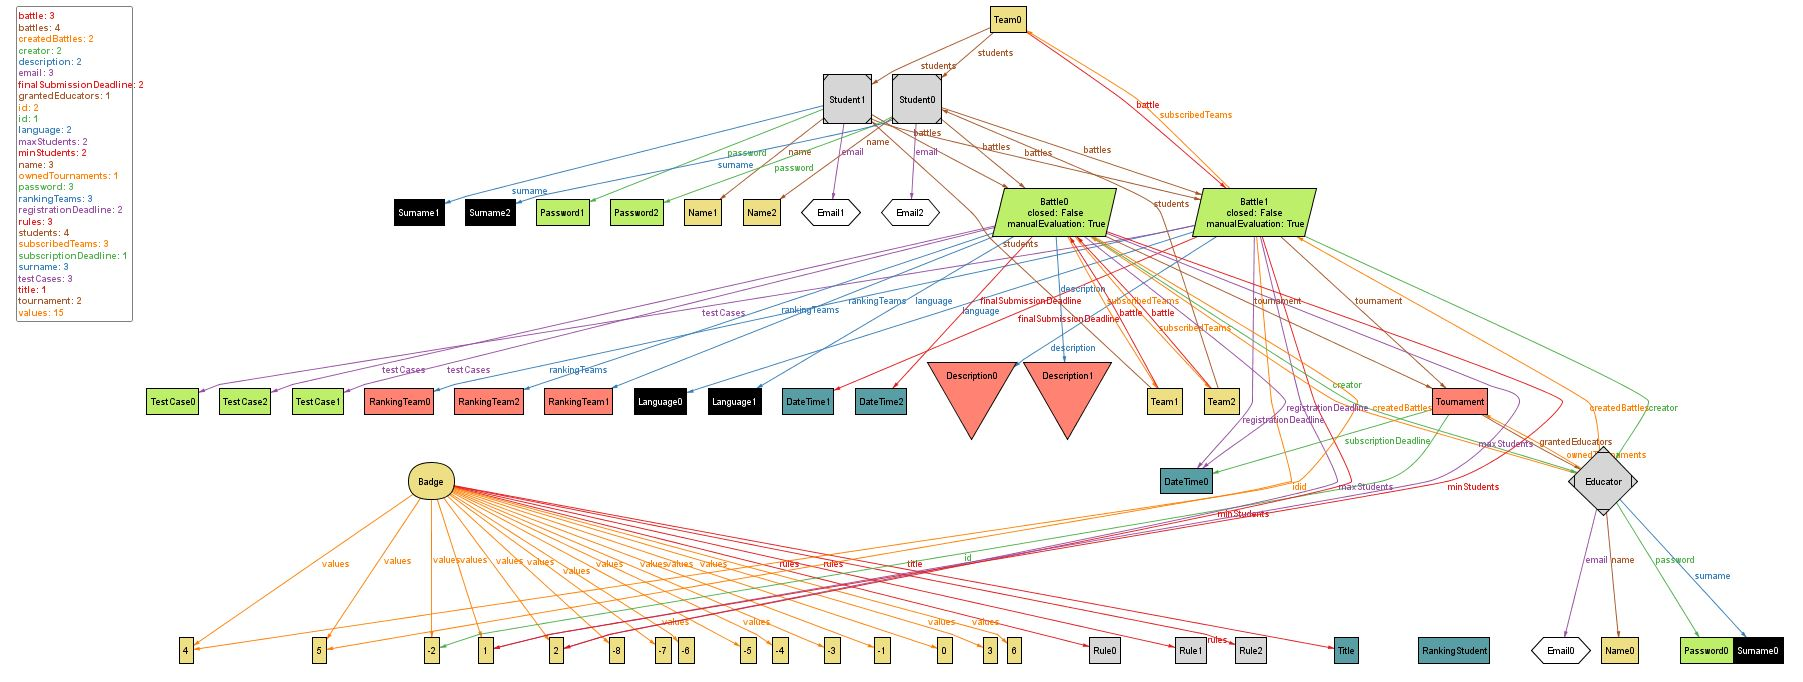
\includegraphics[angle=90,scale = 0.5]{images/alloy/alloy.JPG}
    \caption{World}
\end{figure}
\chapter{Effort Spent}

\section*{Team}

% Please add the number of hours spent for the document in this section*
% To add a new row, copy the following snippet and put it inside the table
% \description_of_the_topic & number_of_hours_spent \\ \hline

\begin{table}[ht]
    \centering
    \begin{tabular}{|l|c|}
        \hline
        \textbf{Topic}                       & \textbf{Time} \\ \hline
        Division of work                     & 2h            \\ \hline
        Revision of chapters 1 and 2         & 2h            \\ \hline
        Definition and division of use cases & 2h30m         \\ \hline
    \end{tabular}
    \caption{Effort Spent during team meetings}
    \label{tab:group-effort-spent}
\end{table}

\section*{Tommaso Pasini}
\begin{table}[ht]
    \centering
    \begin{tabular}{|l|c|}
        \hline
        \textbf{Topic}                      & \textbf{Time} \\ \hline
        Organizaionion document             & 1.5 h         \\ \hline
        Completion and correction chapter 1 & 4h            \\ \hline
    \end{tabular}
    \caption{Effort Spent by Tommaso Pasini}
    \label{tab:pasini-effort-spent}
\end{table}

\section*{Elia Pontiggia}
\begin{table}[ht]
    \centering
    \begin{tabular}{|l|c|}
        \hline
        \textbf{Topic}                                 & \textbf{Time} \\ \hline
        Scenarios                                      & 1h            \\ \hline
        State diagrams                                 & 2h            \\ \hline
        Specific requirements                          & 2h            \\ \hline
        \LaTeX \space document setup and configuration & 2h            \\ \hline
    \end{tabular}
    \caption{Effort Spent by Elia Pontiggia}
    \label{tab:pontiggia-effort-spent}
\end{table}

\section*{Michelangelo Stasi}
\begin{table}[ht]
    \centering
    \begin{tabular}{|l|c|}
        \hline
        \textbf{Topic}          & \textbf{Time} \\ \hline
        Functional Requirements & 2h            \\ \hline
        Domain Assumptions      & 1h30m         \\ \hline
    \end{tabular}
    \caption{Effort Spent by Michelangelo Stasi}
    \label{tab:stasi-effort-spent}
\end{table}


\end{document}